\chapter{Kata Pengantar}
		\begin{figure}[h]
			\centering
			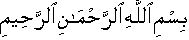
\includegraphics[width=0.5\linewidth]{img/bismillah.png}
		\end{figure}

		Alhamdulillahirabbil’alamin, segala puji bagi Allah SWT, yang telah melimpahkan rahmat dan hidayah-Nya sehingga penulis dapat menyelesaikan Tugas Akhir yang berjudul \textbf{Rancang Bangun Perangkat Lunak \textit{Internet Acces Management} Berbasis Kontainer}. Pengerjaan Tugas Akhir ini merupakan suatu kesempatan yang sangat baik bagi penulis. Dengan pengerjaan Tugas Akhir ini, penulis bisa belajar lebih banyak untuk memperdalam dan meningkatkan apa yang telah didapatkan penulis selama menempuh perkuliahan di Teknik Informatika ITS. Dengan Tugas Akhir ini penulis juga dapat menghasilkan suatu implementasi dari apa yang telah penulis pelajari.
		Selesainya Tugas Akhir ini tidak lepas dari bantuan dan dukungan beberapa pihak. Sehingga pada kesempatan ini penulis mengucapkan syukur dan terima kasih kepada:
		\begin{enumerate}
			\item Allah SWT atas anugerahnya yang tidak terkira kepada penulis dan Nabi Muhammad SAW.
			\item Bapak, Mama, dan keluarga Penulis yang selalu memberikan perhatian, dorongan dan kasih sayang yang menjadi semangat utama bagi diri Penulis sendiri baik selama penulis menempuh masa perkuliahan maupun pengerjaan Tugas Akhir ini.
			\item Bapak Royyana Muslim Ijtihadie, S.Kom., M.Kom., PhD. selaku Dosen Pembimbing yang telah banyak meluangkan waktu untuk memberikan ilmu, nasihat, motivasi, pandangan dan bimbingan kepada Penulis baik selama Penulis menempuh masa kuliah maupun selama pengerjaan Tugas Akhir ini.
			\item Bagus Jati Santoso, S.Kom., PhD. selaku dosen pembimbing yang telah memberikan ilmu, dan masukan kepada Penulis.
			\item Seluruh tenaga pengajar dan karyawan Jurusan Teknik Informatika ITS yang telah memberikan ilmu dan waktunya demi berlangsungnya kegiatan belajar mengajar di Jurusan Teknik Informatika ITS.
			\item Seluruh teman Penulis di Jurusan Teknik Informatika ITS yang telah memberikan dukungan dan semangat kepada Penulis selama Penulis menyelesaikan Tugas Akhir ini.
			\item Teman-teman, Kakak-kakak dan Adik-adik \textit{administrator} Laboratorium Arsitektur dan Jaringan Komputer yang selalu menjadi teman untuk berbagi ilmu.
		\end{enumerate}

		Penulis menyadari bahwa Tugas Akhir ini masih memiliki banyak kekurangan. Sehingga dengan kerendahan hati, penulis mengharapkan kritik dan saran dari pembaca untuk perbaikan ke depannya.

		\hfill Surabaya, Juni 2018 \\ \\
		\hfill Fourir Akbar